\documentclass[procedia]{easychair}
% \usepackage[textwidth=15cm]{geometry}
\usepackage[utf8]{inputenc}
%\usepackage[affil-it]{authblk}
\usepackage{graphicx}
\usepackage{cite}
\usepackage{url}

% This provides the \BibTeX macro
\usepackage{doc}
\usepackage{makeidx}

%opening
% \author[1]{Gijs van den Oord}
% \author[1]{Rena Bakhshi}
% \affil[1]{Netherlands eScience Center}

\title{Parallel Post-Processing of\\ the EC-Earth Climate Model Output}
\titlerunning{Parallel Post-Processing of the EC-Earth Climate Model Output}

\author{
    Gijs van den Oord%\inst{1}
\and
    Rena Bakhshi%\inst{1}
}
 
\institute{
  Netherlands eScience Center,
  Amsterdam, The Netherlands\\
  \email{\{g.vandenoord,r.bakhshi\}@esciencecenter.nl}
\\
 }
 
\authorrunning{van den Oord and Bakhshi}

\begin{document}

\maketitle

\begin{abstract}
The increasing resolution of climate and weather models has resulted in a fast 
growth of their data production. This calls for a more modern and efficient 
approach to the post-processing of these data. We have exploited the 
flexibility of the python language and the parallel nature of the 
post-processing workload to create a new software package to process the output 
of EC-Earth, a coupled atmosphere-ocean 
model. 
\end{abstract}

\section{Introduction}
The ever-growing capability of supercomputers allows us to run sufficiently 
parallelized numerical algorithms at unprecedented scales. Optimized 
fluid-dynamical and atmospheric codes that benefit from the continuous 
increase of processor cache size, instruction vector length and number of 
cores per die enable us to explore dynamical systems at higher 
spatial and temporal resolution, while avoiding a penalty in time and energy 
consumption. For example, it is feasible to let coupled atmospheric-ocean 
models at a resolution of $\sim$10 km simulate 100 years of climate 
evolution, as is currently carried out within the PRIMAVERA joint effort 
\cite{PRIMAVERA} by 
various climate modeling groups among which the EC-Earth \cite{ECEARTHv22} 
consortium.\\
\\
Along with the model resolution the data production rate grows, 
whereas the speed of mass storage systems generally only moderately improve. 
This impacts the I/O performance of these programs \cite{Asif20142370}, in 
particular off-line 
post-processing algorithms which typically exhibit low computational intensity 
and frequent disk access, for example when computing time averages of 
meteorological gridpoint fields. Nevertheless it often remains preferred to 
have a separate post-processing step to keep the high-frequency model output 
accessible for further studies\footnote{This could be also achieved by a 
library aggregating the data in memory during the model run, but 
this functionality is absent in the atmosphere model in EC-Earth}. On the other 
hand, the number of requested post-processed fields has increased significantly 
for the next generation of model intercomparison projects (MIPs) in the climate 
science community \cite{CMIP6}. It is therefore feasible to minimize the 
computation time by 
exploiting the parallel nature of the problem of processing many variables at 
once.\\
\section{Design}
The EC-Earth model output for the PRIMAVERA runs consist of GRIB-files produced 
by the atmosphere component, the Integrated Forecasting System (IFS), and 
netCDF files produced by the coupled ocean model NEMO \cite{NEMO}. The latter 
component 
contains online post-processing capability, provided by the XIOS library. The 
atmospheric output is post-processed with existing technology, the widely used 
Climate Data Operators (CDO) \cite{CDO} to produce netCDF files for all 
requested 
variables. After this step, all variables are extracted from netCDF and sent to 
the CMOR3 library \cite{CMOR} which handles the reformatting to CMIP 
conventions. Using the 
python bindings of these tools allows us to avoid complex bash scripts and 
helps us to create a maintainable codebase.\\
\\
The CMOR library rewrites input data according to a set of rules that are 
encoded in a set of json-files, referred to as \emph{CMOR-tables}. These tables 
contain information about variable names and descriptions, but also the type of 
data reduction that has been applied to high-frequency instantaneous fields. We 
identify the workload as a set of independent tasks that can be executed in 
parallel. Each task consists of a target, a variable in one of the CMOR-tables, 
and a source, a variable inside one of the model output files. The tasks are 
constructed from a given set of desired targets and a fixed lookup table 
containing pairs of source variables and possible targets. The ocean tasks 
are assumed to be post-processed and are sent to the CMOR library right away. 
The atmosphere tasks are grouped in a synchronized queue, and multiple worker 
threads perform the post-processing step. The results of the post-processing 
threads are stored as temporary netCDF files (keeping them in memory is 
currently not supported by CDO), which serve as input for the output rewriting 
step in CMOR. The software supports setting a limit on the diskspace used by 
these temporary files: after reaching this threshold, the batch of processed 
variables will be cmorized and the temporary files are removed.\\
\begin{figure}[ht]
 \centering
 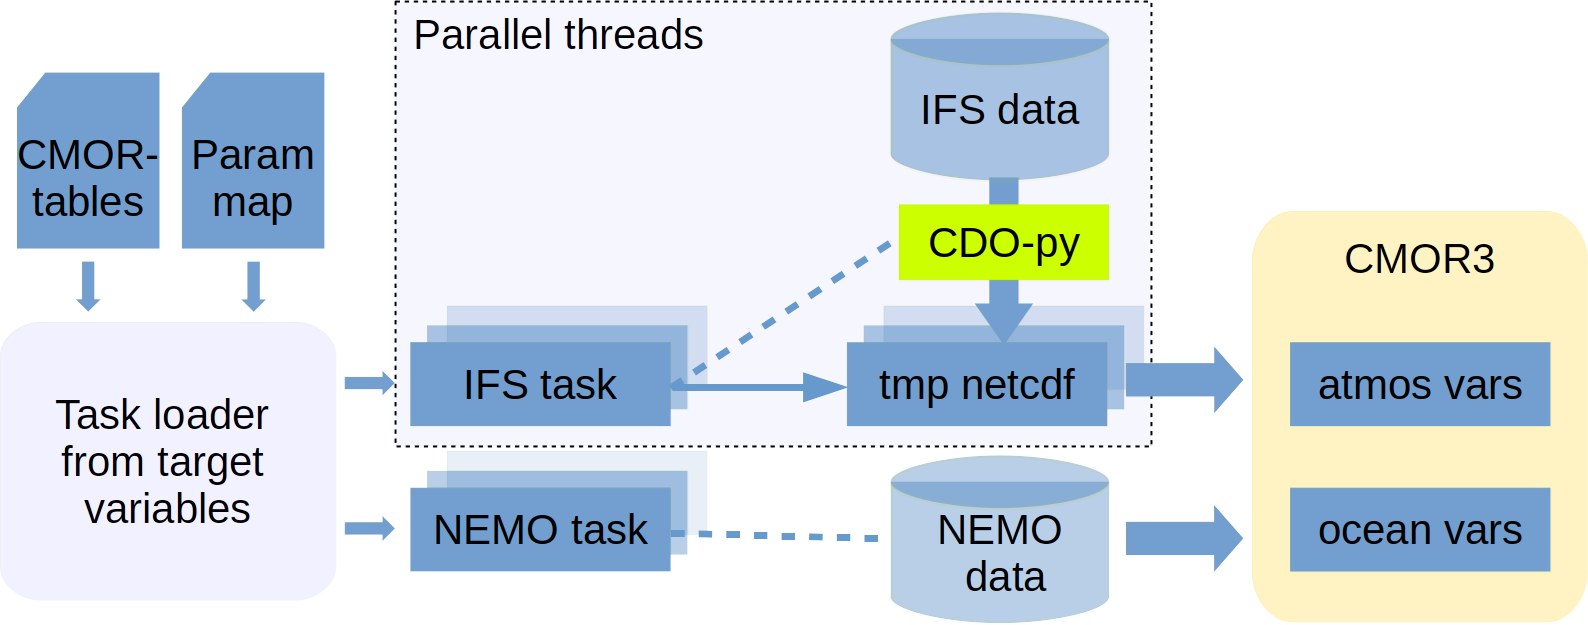
\includegraphics[width=\textwidth,clip]{ece2cmor3flowv3.png}
 \caption{Graph of the data flow in the ece2cmor3 program. The parallelized 
processing is highlighted in the violet box.}
\end{figure}
\\
Throughout the code, hard-coded assumptions about the nature of the resulting 
variables are kept to a minimum. This is important because all information is 
contained in the input tables, which tend to be volatile and will differ for 
various intercomparison studies. Finally we note that a significant speedup has 
been achieved by optimizing the ordering of the CDO operators for data 
reduction. A dynamical field will typically be processed using (i) selection 
criteria for extracting data from the model output, (ii) time aggregation 
operators mapping to lower time resolution and (iii) a grid projection operator 
mapping the data to a regular Gaussian grid\footnote{IFS output is usually 
defined on a reduced gaussian grid or in a spectral representation}. The latter 
step is costly for high-resolution 3D fields, but it is a linear operation 
(matrix multiplication) which commutes with linear time aggregation operators 
such as averaging. Hence it can often be applied as the last step on the 
reduced data.
\section{Results}
The result of our effort is the open source python package \texttt{ece2cmor3}, 
which can be found at \texttt{https://github.com/goord/ece2cmor3}. This code is 
also included in the PRIMAVERA branch of EC-Earth 3.2 and will soon be merged 
to the EC-Earth trunk as a successor of the existing \texttt{ece2cmor} code. 
For benchmarking we focus upon the post-processing of 37 six-hourly 
three-dimensional fields, which constitutes the bulk of the output data 
processing time within the PRIMAVERA project. A single month of 
six-hourly data takes 80GB of disk space, whereas the post-processed temporary  
netCDF files together occupy 68GB. We have run this test on the ECMWF Cray XC40, 
which consists of intel Xeon nodes of the broadwell generation with 18 physical 
cores per node and 128GB of DDR4 memory. As temporary storage we use the scratch 
drive, managed by the parallel LUSTRE file system.\\
\\
\begin{figure}[b]
 \centering
 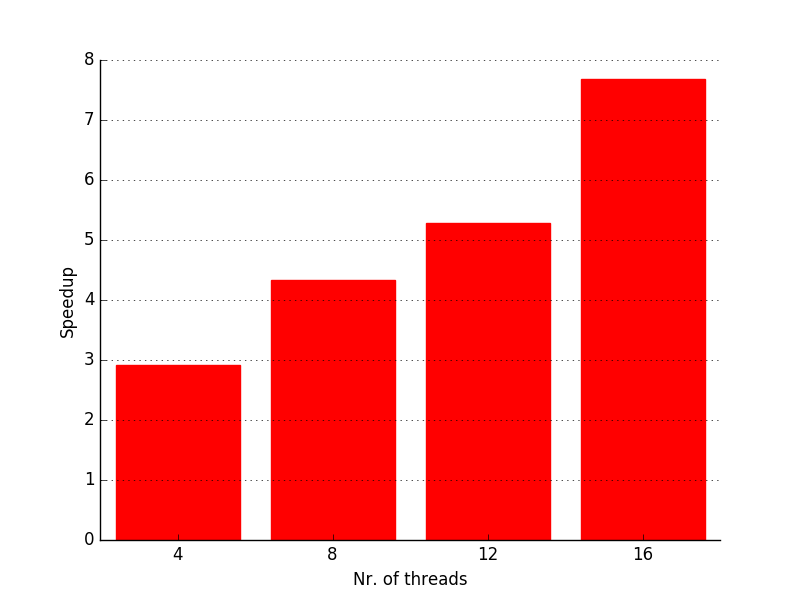
\includegraphics[width=0.5\textwidth]{speedup_chart.png}
 \caption{Speedup of the post-processing workload with multiple threads 
processing independent climate fields.}
\end{figure}
The single-threaded version takes 2.5 hours to finish processing a month 
six-hourly atmosphere data on this system, which is much slower than the 
simulation itself. By launching 16 worker threads we can achieve a speedup of 
almost a factor of eight. The scaling behavior can be explained by the finite 
bandwidth to the temporary storage and the fact that CDO itself has been 
configured to run four threads per processing task. Eventually we can also 
partition the workload into multiple chunks of variables that can be executed 
on different nodes if further acceleration is needed.
\section{Conclusion and Outlook}
We have written a package for processing the output of EC-Earth that is 
flexible, maintainable and achieves a good performance by parallelizing the 
most time-consuming part of the workload. It is expected to perform its duty in 
EC-Earth for the upcoming CMIP6 model runs. However, this exercise would have 
been avoided if the atmosphere model had been linked to an on-line 
postprocessing library such as XIOS or some library version of CDO. This will 
be a necessary step to increase space and time resolutions further in future 
climate simulations. Such a software component will have to contain highly 
optimized grid mapping algorithms and support parallel processing of multiple 
atmospheric fields.


%------------------------------------------------------------------------------
% Refs:
%
\label{sect:bib}
\bibliographystyle{plain}
%\bibliographystyle{alpha}
%\bibliographystyle{unsrt}
%\bibliographystyle{abbrv}
\bibliography{citations}

%------------------------------------------------------------------------------

\end{document}
